	%-----------------Aggregation des liens ----------%
				\citep{buehrer2008scalable} ont exploité l'existence de plusieurs ensembles de pages web qui ont les même liens sortants. S'intitulant  VNM pour Virtual Node Miner, leurs approche est basée sur la réduction du nombre de liens en créant des nouveaux sommets virtuels qui sont ajoutés au graphe. Soit G = (V,E) un graphe orienté, l'algorithme proposé se compose de deux phases essentielles :
				\begin{enumerate}
				
				
					\item \textbf{Phase de Clustering :}
					
					Le but de cette première étape est de contourner la tâche presque impossible d'extraction simultanée de centaines de millions de points de données en groupant d'abord les sommets similaires dans le graphes dans des clusters. 
				Pour cela k fonctions de hachage indépendantes sont utilisées pour obtenir une matrice de taille V * k. Par la suite, les lignes de la matrice  sont triées lexicographiquement
				%Ce tri est assez rapide car il ne nécessite que O (2V log V) en mémoire à la fois, ce qui tient dans la RAM (ou nous le faisons en minant le graphique en morceaux). 
				et elle est parcourue colonne par colonne en regroupant les lignes ayant la même valeur. Lorsque le nombre total de lignes chute au-dessous d'un seuil ou que le bord de la matrice de hachage est atteint, les identifiants des sommets associés aux lignes sont renvoyé au processus d'extraction (Phase 02). 
					
					\item \textbf{Phase d'Extraction de Motifs :}				Le but de cette étape est de localiser des sous-ensembles communs de liens sortants dans les sommets donnés. 
				Ainsi les ensembles plus grands et fréquents présentent un intérêt, car ils peuvent représenter des motifs plus pertinents et une meilleure compression. En effet, les performances de compression d'un motif  sont calculés en fonction de sa fréquence dans la liste d'adjacence, et de sa taille qui est le nombre de liens qu'il contient \eqref{eqcompperf}.
				%%% Formule
				\begin{equation}
				Compression(P)=(P.fréquence-1)(P.taille-1)-1
				\label{eqcompperf}
				\end{equation}
				Afin d'extraire ces motifs, VNM utilise une heuristique gloutonne. Cette heuristique procède comme suit :
				\begin{enumerate}
				\item Extraire un histogramme des identifiants de liaison sortante à partir de la liste d'adjacence des sommets données.
				\item Les listes sont réorganisées dans l'ordre décroissant des fréquences des liens sortants en éliminant ceux qui apparaissent une seul fois uniquement.
				\item Chaque lien sortant est ajouté à un arbre de préfixes avec l'ensemble trié de ces extrémités initiales selon leurs identifiants. 
				\item L'arbre est par la suite parcouru afin d'identifier les motifs qui maximisent la formule de performance de la compression \ref{eqcompperf}. Ces motifs sont ensuite convertis en nœuds virtuels et les identificateurs de sommet de leurs listes sont supprimés.
				\end{enumerate}
				 
				\end{enumerate}
				
				L'algorithme est appliqué jusqu'à ce que la réduction n'apporte pas un gain significative. La figure \ref{tab:VNM_exm} illustre le principe de fonctionnement de cette méthode sur un exemple.
				
				
			%%%%		Inclure un exemple 
			
		\begin{table}[h!]
			
		 \begin{flushleft}
			\begin{tabular}{C{4cm}||C{9cm} }
				 Phase 01 &  Phase 02 \\
				 {\renewcommand{\arraystretch}{0.6}
					\begin{tabular}[b]{R{0.4cm}|L{0.3cm} L{0.3cm} L{0.3cm}}
				 			id & \(\displaystyle h_{1}\)  & \(\displaystyle h_{2}\) &  \(\displaystyle h_{3}\) \\
							\hline  13 &\cellcolor{blue!25}10&\cellcolor{blue!25}11&\cellcolor{blue!25}12\\
							    	    23 &\cellcolor{blue!25}10&\cellcolor{blue!25}11&\cellcolor{blue!25}12\\
								   	43 &\cellcolor{blue!25}10&\cellcolor{blue!25}11&\cellcolor{blue!25}12\\
				  					55 &\cellcolor{blue!25}10&\cellcolor{blue!25}11&\cellcolor{blue!25}12\\
				  					64 & \cellcolor{blue!25}10&\cellcolor{blue!25}11&\cellcolor{blue!25}12\\
				  					102 &\cellcolor{blue!25}10&\cellcolor{blue!25}11&\cellcolor{blue!25}12\\
				  					204 &\cellcolor{blue!25}10&\cellcolor{blue!25}11&\cellcolor{blue!25}12\\
				  					431 &\cellcolor{blue!25}10&\cellcolor{blue!25}11&\cellcolor{blue!25}12\\
				  					480 &\cellcolor{blue!25}10&\cellcolor{blue!25}11&2\\
				  					501 &\cellcolor{blue!25}10&4&1\\
			\end{tabular}
				
				
				
				1. Calcul des fonctions de hachage et groupement des sommets			
			} &
			{
				 \begin{multicols}{2}
					\renewcommand{\arraystretch}{0.6}
 						 \begin{tabular}{R{0.4cm}|L{3.2cm} }
				 id &  liens sortants \\\hline
				  13 & 1 2 3 8\\
				  23 & 1 2 3 5 6 10 12 15 \\
				  43 & 1 2 3 5 6 10 22 31\\
				  55 & 1 2 3 5 \\
				  64 & 1 2 3 5 6 10 12 15 \\
				  102 & 1 2 3 20\\
				  204 & 1 7 8 9\\
				  431 & 1 2 3 4 5 6 10 22 31\\
			\end{tabular}
			
			
			2.1 la Liste d'adjacence.
			\columnbreak
 				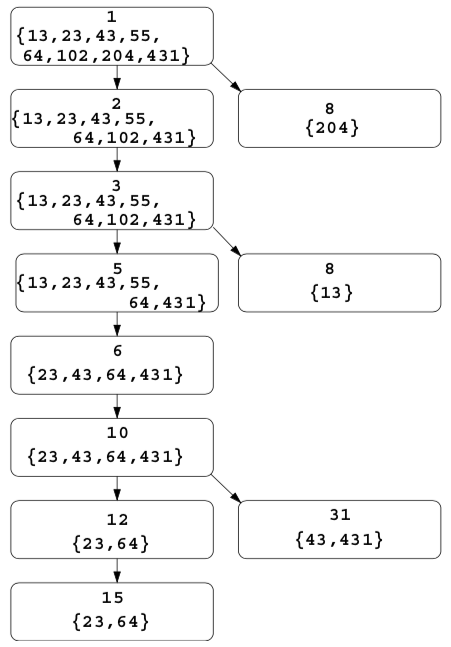
\includegraphics[scale=0.3]{ressources/image/VNM_exemple.png} 
 			%	2.2 Construction de l'arbre
 			
			\end{multicols}
			\begin{center}
		\renewcommand{\arraystretch}{0.6}
		\begin{tabular}{C{1cm} | C{1cm} L{4cm} C{1cm}}
			taille & freq & Liste des noeuds & Savings\\\hline
			6&4&43 431 23 64&14\\
			3&7&23 55 102 64 43 431&11\\
			8&2&23 64&6\\
			7&2&43 431&5\\
		
				\end{tabular}
				2.3 Extraction des Motifs
		\end{center}
			}
			
			\end{tabular}
		\end{flushleft}
		\caption{Exemple d'exécution de VNM}
   			 \label{tab:VNM_exm}
		\end{table}
		
		%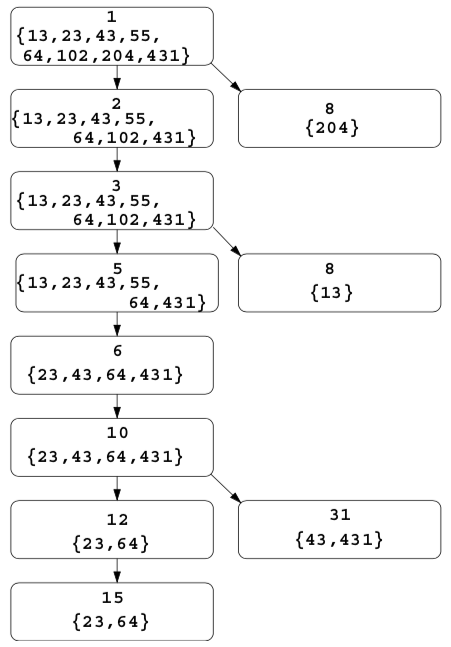
\includegraphics[scale=0.5]{ressources/image/VNM_exemple.png}